\documentclass[11pt]{article}
\usepackage{amssymb}
\usepackage{amsthm}
\usepackage{enumitem}
\usepackage{physics,amsmath}
\usepackage{bm}
\usepackage{adjustbox}
\usepackage{mathrsfs}
\usepackage{graphicx}
\usepackage{siunitx}
\usepackage[mathscr]{euscript}

\title{\textbf{Solved selected problems of Classical Mechanics - Gregory}}
\author{Franco Zacco}
\date{}

\addtolength{\topmargin}{-3cm}
\addtolength{\textheight}{3cm}

\newcommand{\hatr}{\bm{\hat{r}}}
\newcommand{\hatx}{\bm{\hat{x}}}
\newcommand{\haty}{\bm{\hat{y}}}
\newcommand{\hatz}{\bm{\hat{z}}}
\newcommand{\hatn}{\bm{\hat{n}}}
\newcommand{\hati}{\bm{\hat{i}}}
\newcommand{\hatj}{\bm{\hat{j}}}
\newcommand{\hatk}{\bm{\hat{k}}}
\newcommand{\uvi}{\bm{i}}
\newcommand{\uvj}{\bm{j}}
\newcommand{\uvk}{\bm{k}}
\newcommand{\hatth}{\bm{\hat{\theta}}}
\newcommand{\hatphi}{\bm{\hat{\phi}}}
\newcommand{\hatrho}{\bm{\hat{\rho}}}
\newcommand{\ngrad}[1]{\text{grad}_{\bm{#1}}}

\theoremstyle{definition}
\newtheorem*{solution*}{Solution}
\renewcommand*{\proofname}{\bf{Solution}}

\begin{document}
\maketitle
\thispagestyle{empty}

\section*{Chapter 19 - Problems in rigid body dynamics}

\begin{proof}{\textbf{19.1}}
    Let us consider the following system
    \begin{center}
        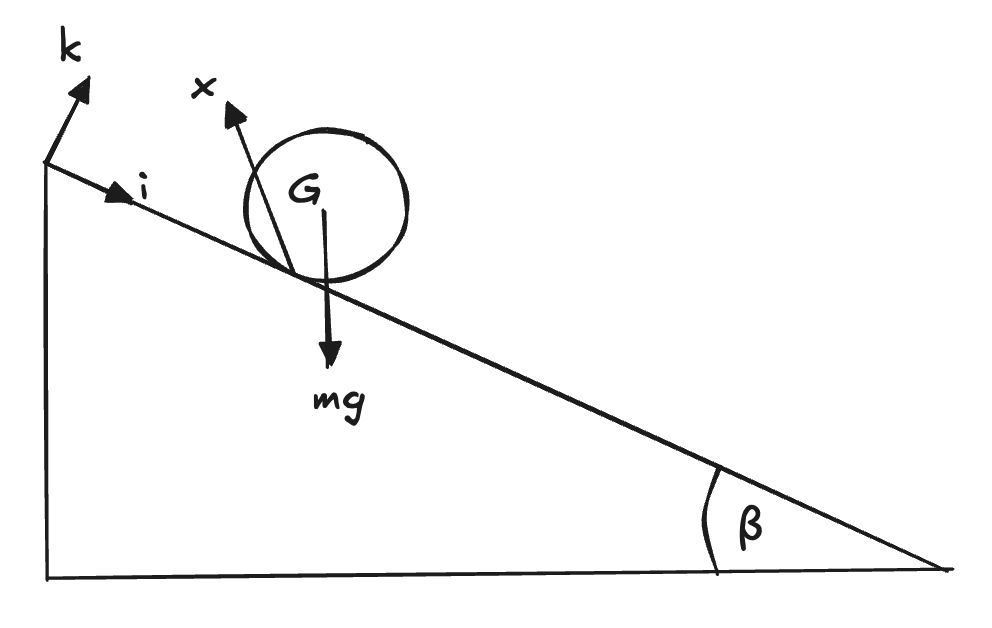
\includegraphics[scale=0.3]{ch19-1.png}
    \end{center}
    Then from the governing equations we have that
    \begin{align*}
        m\bm{\dot{V}} &= \bm{X} + mg\sin\beta\bm{i} - mg\cos\beta\bm{k}\\
        \bm{\dot{L}}_G &= (-b\bm{k}) \times \bm{X} 
    \end{align*}
    Where $\bm{X}$ is the reaction of the table exerted on the ball.
    Using that $\bm{L}_G = A\bm{\omega}$ and eliminating the reaction $\bm{X}$
    we get that
    \begin{align*}
        A\bm{\dot{\omega}}
        &= (-b\bm{k})
        \times (m\bm{\dot{V}} - mg\sin\beta\bm{i} + mg\cos\beta\bm{k})\\
        &= b(m\bm{\dot{V}} - mg\sin\beta\bm{i} + mg\cos\beta\bm{k})
        \times \bm{k}\\
        &= mb\bm{\dot{V}}\times\bm{k} - mgb\sin\beta\bm{i}\times \bm{k}\\
        &= mb\bm{\dot{V}}\times\bm{k} + mgb\sin\beta\bm{j}
    \end{align*}
    On integrating with respect to $t$ we get that
    \begin{align*}
        A\bm{\omega} + mb\bm{k}\times\bm{V} &= \bm{C} + mgbt\sin\beta\bm{j}
    \end{align*}
    Where $\bm{C}$ is a constant vector. In particular if we take the scalar
    product of this equation with $\bm{k}$, we have that
    \begin{align*}
        A\bm{\omega}\cdot\uvk + mb(\bm{k}\times\bm{V})\cdot\uvk
        &= \bm{C}\cdot\uvk + mgbt\sin\beta\bm{j}\cdot\uvk\\
        A\bm{\omega}\cdot\uvk &= n
    \end{align*}
    Where $n$ is a constant. Also, we used that $\uvj \cdot \uvk = 0$ and 
    the triple product is also 0. Therefore we see that the component of
    $\bm\omega$ in the direction of $\uvk$ (perpendicular to the inclined
    plane) is constant independent of the motion of the ball.

    If we now consider that the ball is rolling, then the particle $C$ in
    contact with the plane has zero velocity, so the rolling condition give us
    \begin{align*}
        \bm{V} + b\uvk \times \bm{\omega} = \bm{0}
    \end{align*}
    Now, by cross-multiplying the conservation principle by $\uvk$ we have that 
    \begin{align*}
        A\uvk \times \bm{\omega}
        &= \uvk \times \bm{C} + mgbt\sin\beta\uvk\times\uvj
        - mb\uvk \times(\bm{k}\times\bm{V})\\
        &= \uvk \times \bm{C} - mgbt\sin\beta\uvi
        - mb((\uvk\cdot\bm{V})\uvk - (\uvk\cdot\uvk)\bm{V})\\
        &= \uvk \times \bm{C} - mgbt\sin\beta\uvi + mb\bm{V}
    \end{align*}
    Therefore by joining this equation and the rolling condition equation
    we get that 
    \begin{align*}
        \bm{V} + \frac{mb^2}{A}\bm{V}
        &= -\frac{b}{a}\uvk \times \bm{C} + mgbt\sin\beta\uvi\\
        \bm{V} + \frac{mb^2}{A}\bm{V}
        &= \frac{b}{a}\bm{C}\times\uvk + mgbt\sin\beta\uvi
    \end{align*}
    This shows that $\bm{V}$ is dependent on time. If
    we integrate again this equation we see that the rolling motion
    depends on $t^2$ and therefore the path of the ball must be a parabola.  
\end{proof}
\cleardoublepage
\begin{proof}{\textbf{19.2}}
    Let us consider the following system
    \begin{center}
        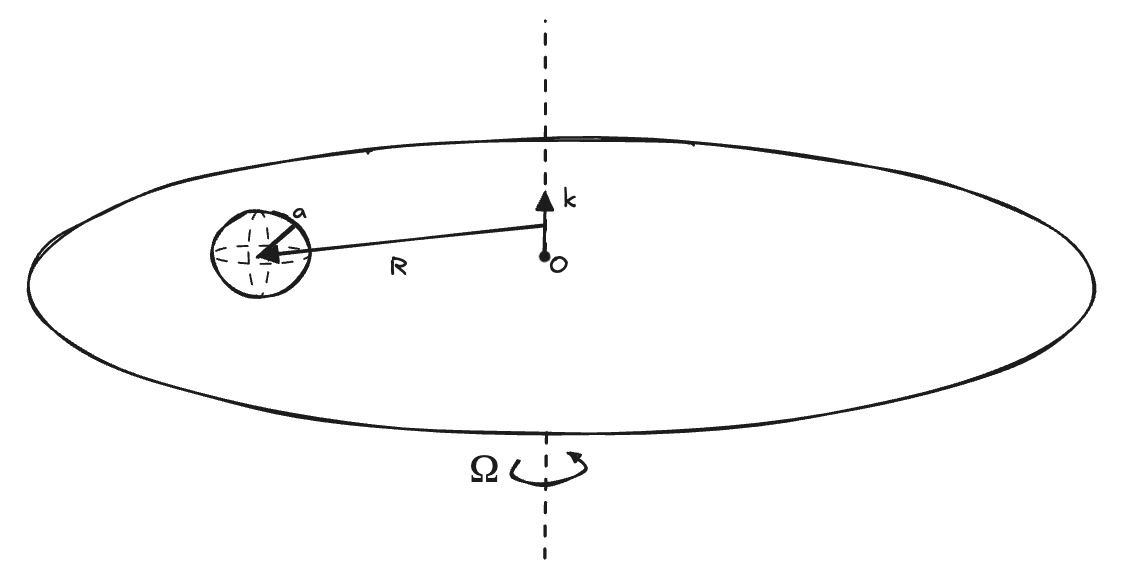
\includegraphics[scale=0.3]{ch19-2.png}
    \end{center}
    Then from the governing equations we have that
    \begin{align*}
        m\bm{\dot{V}} &= \bm{X} - mg\bm{k}\\
        \bm{\dot{L}}_G &= (-a\bm{k}) \times \bm{X} 
    \end{align*}
    Where $\bm{X}$ is the reaction of the turntable exerted on the ball.
    Using that $\bm{L}_G = A\bm{\omega}$ where $A = \frac{2}{5}ma^2$ is the
    moment of inertia of the ball, then eliminating the reaction $\bm{X}$
    we get that
    \begin{align*}
        A\bm{\dot{\omega}}
        &= (-a\bm{k})
        \times (m\bm{\dot{V}} + mg\bm{k})\\
        &= a(m\bm{\dot{V}} + mg\uvk)
        \times \bm{k}\\
        &= ma\bm{\dot{V}}\times\bm{k}
    \end{align*}
    On integrating with respect to $t$ we get that
    \begin{align*}
        A\bm{\omega} + ma\bm{k}\times\bm{V} &= \bm{C}
    \end{align*}
    Where $\bm{C}$ is a constant vector. In particular if we take the scalar
    product of this equation with $\bm{k}$, we have that
    \begin{align*}
        A\bm{\omega}\cdot\uvk + ma(\bm{k}\times\bm{V})\cdot\uvk
        &= \bm{C}\cdot\uvk\\
        A\bm{\omega}\cdot\uvk &= n
    \end{align*}
    Where $n$ is a constant. Also, we used that the triple product is also 0.
    Therefore we see that in any motion of the ball, the vertical spin
    $\bm{\omega}\cdot\uvk$ is constant.

    If we now consider that the ball is rolling, then the particle $C$ in
    contact with the turntable has zero velocity, so the rolling condition give
    us
    \begin{align*}
        \bm{V}_C = \bm{V} + a\uvk \times \bm{\omega} = \bm{0}
    \end{align*}
    Also, from the equation for $A \bm{\dot\omega}$ we derived above, replacing
    the value of $A$ we have that
    \begin{align*}
        \frac{2}{5}ma^2\bm{\dot{\omega}}
        &= ma\bm{\dot{V}}\times\bm{k}\\
        \frac{2}{5}a\bm{\dot{\omega}}
        &= \bm{\dot{V}}\times\bm{k}
    \end{align*}
    And cross-multiplying this equiation by $\uvk$ we obtain an expression for
    $\bm{\dot V}$ as follows
    \begin{align*}
        \frac{2}{5}a\uvk \times \bm{\dot{\omega}}
        &= \uvk \times(\bm{\dot{V}}\times\bm{k})\\
        \frac{2}{5}a\uvk \times \bm{\dot{\omega}}
        &= \bm{\dot{V}} (\uvk\cdot\uvk) - \uvk(\uvk\cdot\bm{\dot{V}})\\
        \frac{2}{5}a\uvk \times \bm{\dot{\omega}}
        &= \bm{\dot{V}}
    \end{align*}
    If we assume the position of the ball's center of mass is determined by a
    vector $\bm{R}$ from the axis $\{O, \uvk\}$ then the velocity $\bm V_C$
    of the particle $C$ is also
    \begin{align*}
        \bm{V}_C = \Omega\uvk \times \bm{R}
    \end{align*}
    Hence by joining the rolling condition and this equation we have that
    \begin{align*}
        \bm{V} + a\uvk \times \bm{\omega} &= \Omega\uvk \times \bm{R}
    \end{align*}
    Derivating this expression and replacing the value for
    $a\uvk \times \bm{\dot\omega}$ we finnally get that
    \begin{align*}
        \bm{\dot V} + \frac{5}{2}\bm{\dot V} &= \Omega\uvk \times \bm{V}\\
        \frac{7}{2}\bm{\dot V} &= \Omega\uvk \times \bm{V}\\
        \bm{\dot V} &= \frac{2}{7}\Omega\uvk \times \bm{V}
    \end{align*}
    Integrating this equation we get that
    \begin{align*}
        \bm{\dot R} &= \frac{2}{7}\Omega\uvk \times \bm{R} + \bm{C}
    \end{align*}
    Where $\bm{C}$ is some constant vector.

    Finally, let us suppose that the unit vector $\uvi$ is in the direction of
    $\bm{R}$ at the moment the ball is released. Then by the initial conditions
    we see that $\bm{R} = b\uvi$ and $\bm{\dot{R}} = \Omega b\uvj$ since the
    ball is at rest with respect to the turntable so the constant of
    integration becomes
    \begin{align*}
        \Omega b\uvj &= \frac{2}{7}\Omega b\uvj + \bm{C}\\
        \bm{C} &= \Omega b\bigg(1 -\frac{2}{7}\bigg)\uvj\\
        \bm{C} &= \frac{5}{7}\Omega b\uvj
    \end{align*}
    Therefore
    \begin{align*}
        \bm{\dot R} &= \frac{2}{7}\Omega \uvk \times \bm{R}
        + \frac{5}{7}\Omega b\uvj
    \end{align*}
    To solve this equation let us introduce a new variable $\bm{A}$ defined as
    $$\bm{A} = (\bm{R} + \frac{5}{2} b\uvi)$$
    Hence
    \begin{align*}
        \bm{\dot{A}} &= \frac{2}{7}\Omega \uvk \times \bm{A}
    \end{align*}
    So now we can solve this equation by assumming that 
    $\bm{A} = A_x\uvi + A_y\uvj$ and 
    $\bm{\dot{A}} = \dot{A_x}\uvi + \dot{A_y}\uvj$ as follows
    \begin{align*}
        \dot{A_x}\uvi + \dot{A_y}\uvj
        &= \frac{2}{7}\Omega \uvk \times (A_x\uvi + A_y\uvj)\\
        \dot{A_x}\uvi + \dot{A_y}\uvj
        &= \frac{2}{7}\Omega A_x \uvj - \frac{2}{7}\Omega A_y\uvi
    \end{align*}
    Therefore we get the following system of differential equations
    \begin{align*}
        \dot{A_x} &= -\frac{2}{7}\Omega A_y\\
        \dot{A_y} &= \frac{2}{7}\Omega A_x
    \end{align*}
    Where the solution is 
    \begin{align*}
        A_x &= C_1\cos(\frac{2}{7}\Omega t) - C_2\sin(\frac{2}{7}\Omega t)\\
        A_y &= C_1\sin(\frac{2}{7}\Omega t) - C_2\cos(\frac{2}{7}\Omega t)
    \end{align*}
    When we apply the initial conditions we get that 
    \begin{align*}
        \frac{7}{2}b &= C_1 \qquad 0 = C_2
    \end{align*}
    Therefore
    \begin{align*}
        A_x &= \frac{7}{2}b\cos(\frac{2}{7}\Omega t)\\
        A_y &= \frac{7}{2}b\sin(\frac{2}{7}\Omega t)
    \end{align*}
    But returning to the original variable we get that
    \begin{align*}
        R_x &= \frac{7}{2}b\cos(\frac{2}{7}\Omega t) - \frac{5}{2}b\\
        R_y &= \frac{7}{2}b\sin(\frac{2}{7}\Omega t)
    \end{align*}
    These are the equations for a circular path which has a centre displaced
    $\frac{5}{2}b$ from $O$ and has a radius of $\frac{7}{2}b$.


\end{proof}
\end{document}

















